\section{Implementation}

This section describes the internals of the implementation in more
detail.  It is important to remember that these details are entirely
hidden by the PUSH shell so users and their applications are never
really exposed to the complexity expressed herein.  It is possible
to provide alternate front-ends to the underlying Brasil infrastructure
and applications may choose to interact directly with it and its control
interfaces, but it is not expected that this will be the default mode of 
operation.

\subsection{Interface}

The external interface to our infrastructure is a synthetic file system
much like the interface to the Xcpu~\cite{lucho-xcpu} workload distribution
system.  
Figure \ref{fig:xcpu3Local} gives the the high-level view of the hierarchy 
of the Brasil namespace.


\begin{figure}[htp]
\centering
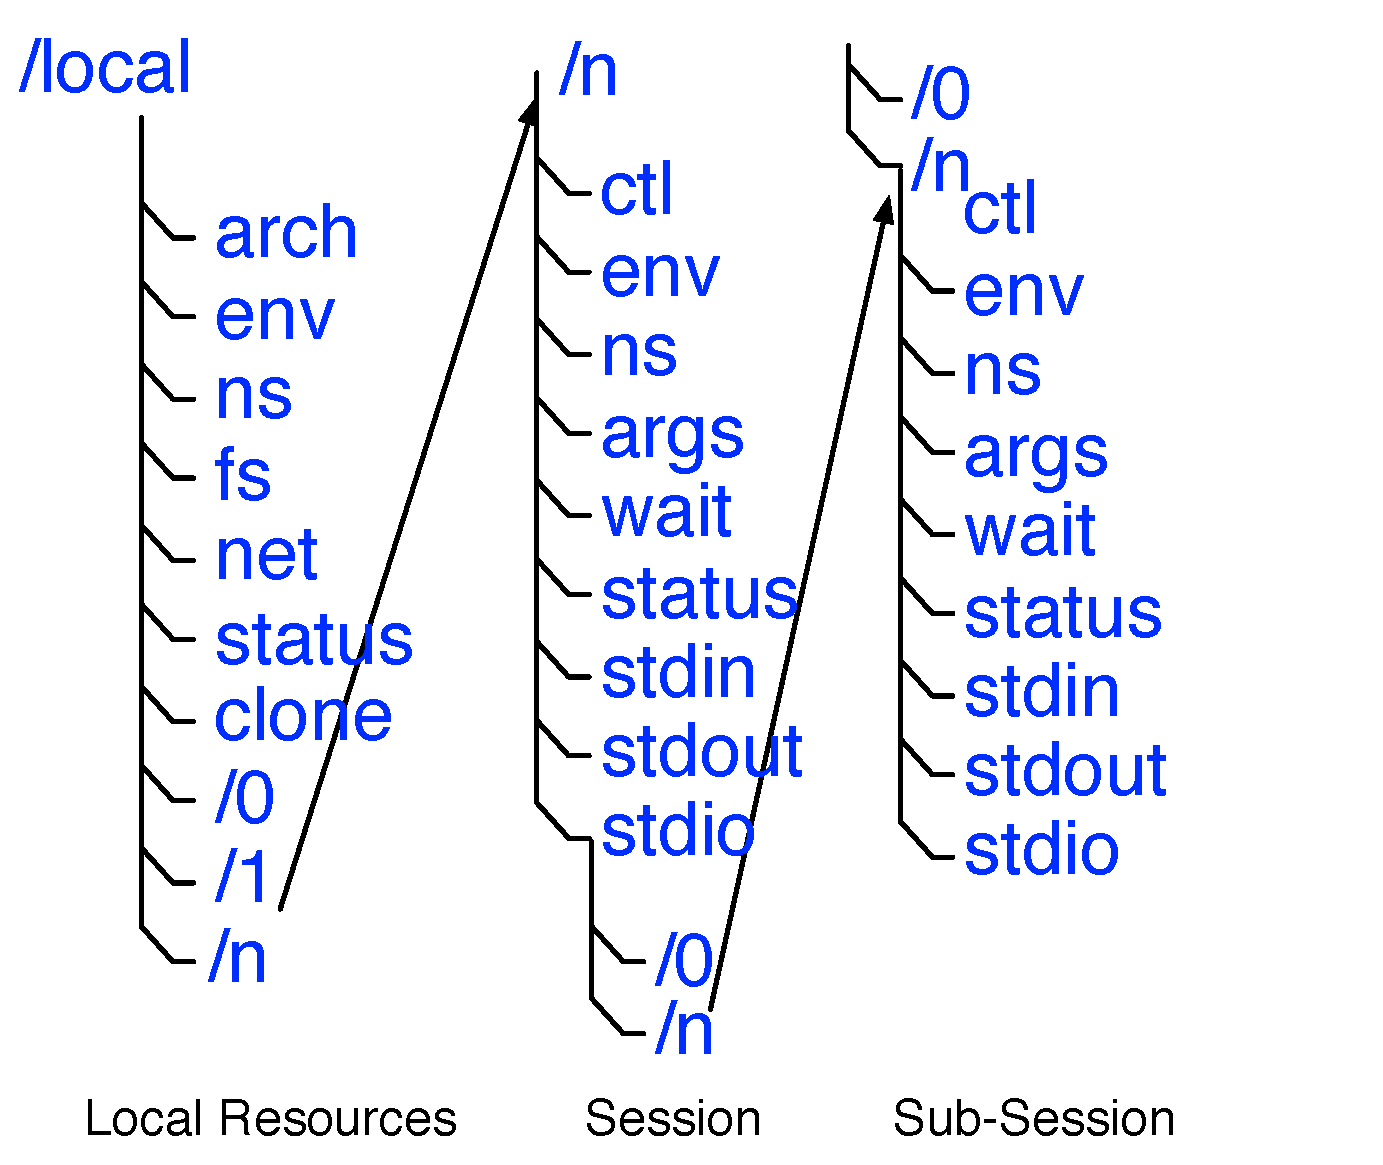
\includegraphics[width=3in]{./img/taskfs-hierarchy.eps}
\caption{Filesystem interface in Brasil}
\label{fig:xcpu3Local}
\end{figure}

Each node in the system has a \emph{local} directory in the root of their
namespace which contains pointers to the resources
available on the node and control files which allows managing 
jobs deployed on the node.
A few files here provide information about the system, like the
\texttt{[arch]} file which tells the architecture and operating system of 
the node while the \texttt{[status]} file provides information about total 
amount of resources currently available, including the remote resources which 
are directly or indirectly decedents of this node.  
Files like \texttt{[env]} and \texttt{[ns]}
allow controlling the default environment and the namespace of the processes
created on this node.  \texttt{[fs]} and \texttt{[net]} are links to the local
filesystem and networking resources available on the node.  The
\texttt{[clone]} file provides the interface to create new sessions which is
the unit of the workload management.

The sessions are represented as directories with the session-id number as 
the directory name.
Each directory is  self-contained and provides interfaces to manage the
execution of the session.  Files like \texttt{[env]} and \texttt{[ns]} are
present in the session directory also, and can be used to overwrite the 
default environment and namespace specifically for this session.  
The \texttt{[ctl]} file is used for controlling the execution and 
the \texttt{[stdio]} file is used to manipulate standard input and output.  

Since sessions themselves can have children, each session directory may have
subsession directories with similar files.  The files at the session directory
level provide the aggregate interfaces to the sub-session directory.

%Whenever any session receives the reservation request, it evaluates it by 
%considering, if it can execute locally or it should break it and divide 
%between its available children.  Depending on the decision,
%it can play one of the following two roles.
%\begin{enumerate}
%  \item \textbf{Execution session}: When the reservation requested is 
%  small enough, the session performs all the requested operations locally.  
%  
%  \item \textbf{Aggregation session}: When request is bigger than what session
%  can handle, it divides the request between children nodes.  The session does
%  this by creating new session and sending the divided
%  reservation request to the each child node available in it's \textbf{CSRV}
%  hierarchy.  These newly created sessions will be binded as directories in the
%  directory of the current session hence making them the sub-sessions of the
%  current session.  The current session now acts as in aggregation point for
%  these sub-sessions by passing the any execution request or input to all
%  sub-sessions and merging the output from all sub-sessions to produce the final
%  output.  These aggregation sessions constitute the non-leaf nodes in the
%  session tree.
%\end{enumerate}
%This way, recursive tree of sessions is created whenever new reservation request
%is received.  This tree of the session is then used to request the execution and
%collect back the results.  This design not only distributes the actual
%execution, but also it distributes the distribution and aggregation process as
%this work is divided between all aggregation sessions.

\subsection{Brasil}

The core of Brasil is a self-contained daemon which is based on a fork of
Inferno~\cite{dorward1997ios}.
Inferno is an open source distributed operating system 
which is a direct descendant of the Plan 9 operating system~\cite{pike1995pbl}.  
It runs natively on
multiple hardware platforms and can also run as a user-space application on
top of other operating systems.
Brasil is based on the hosted version of the Inferno platform.

The Brasil namespace is exported using the \texttt{9P} protocol. 
This protocol is used by Plan 9 and Inferno extensively to access any file. 
Recently the Linux kernel has added support for the \texttt{9P}
protocol\cite{graverobbers}.  This allows Linux to mount filesystems
exported over the 9P protocol.  Other Unix based operating systems can use
FUSE for accessing the 9P based filesystems. 

The applications interact with this mounted Brasil filesystem using the native
filesystem interfaces (e.g. VFS for Linux). Any interaction with this Brasil
filesystem is communicated to Brasil using \textit{9P}. 
If needed, it uses services from the host operating system or from other Brasil
filesystems deployed on remote locations.  The Brasil filesystem then sends the
prepared response over 9P. The host operating system will relay this response
back to the application via the local filesystem interface.

\subsection{Central Services}

The ability to configure many Brasil nodes into hierarchy is provided by the
\textit{central services}.  Contrary to the name, central services is
highly distributed and every Brasil runs an independent instance of the central
services.  

The central services synthetic file server which provides a simple hierarchy of
directory mount points representing remote nodes.  Mounts of the remote nodes
or binds of previously mounted remote nodes are accomplished within this file
system such that anyone who mounts our namespace can also see (and
access) anyone we have mounted transitively,  in such a way a child
node can access a parent nodes, other children, or the parents nodes
parent and so forth. Any node could establish themselves within a
hierarchy by binding a parent's central service directory to the name
\texttt{[/csrv/parent]} and then tell the parent to back-mount their name space
(allowing two way traversal).  In this way children register with parents
triggering the cross-mounts and establishing a two way link between them. Each
Brasil instance needs only to know the information about its parent and children
in the hierarchy and all Brasil nodes initiate these connections leading to
the distributed creation of the Brasil node hierarchy.
 
Figure \ref{fig:xcpu3FSTopo} tries to give a simple overview of how this 
synthetic filesystem view is populated based on the underlying mount
connections between the nodes.

\begin{figure}[htp]
\centering
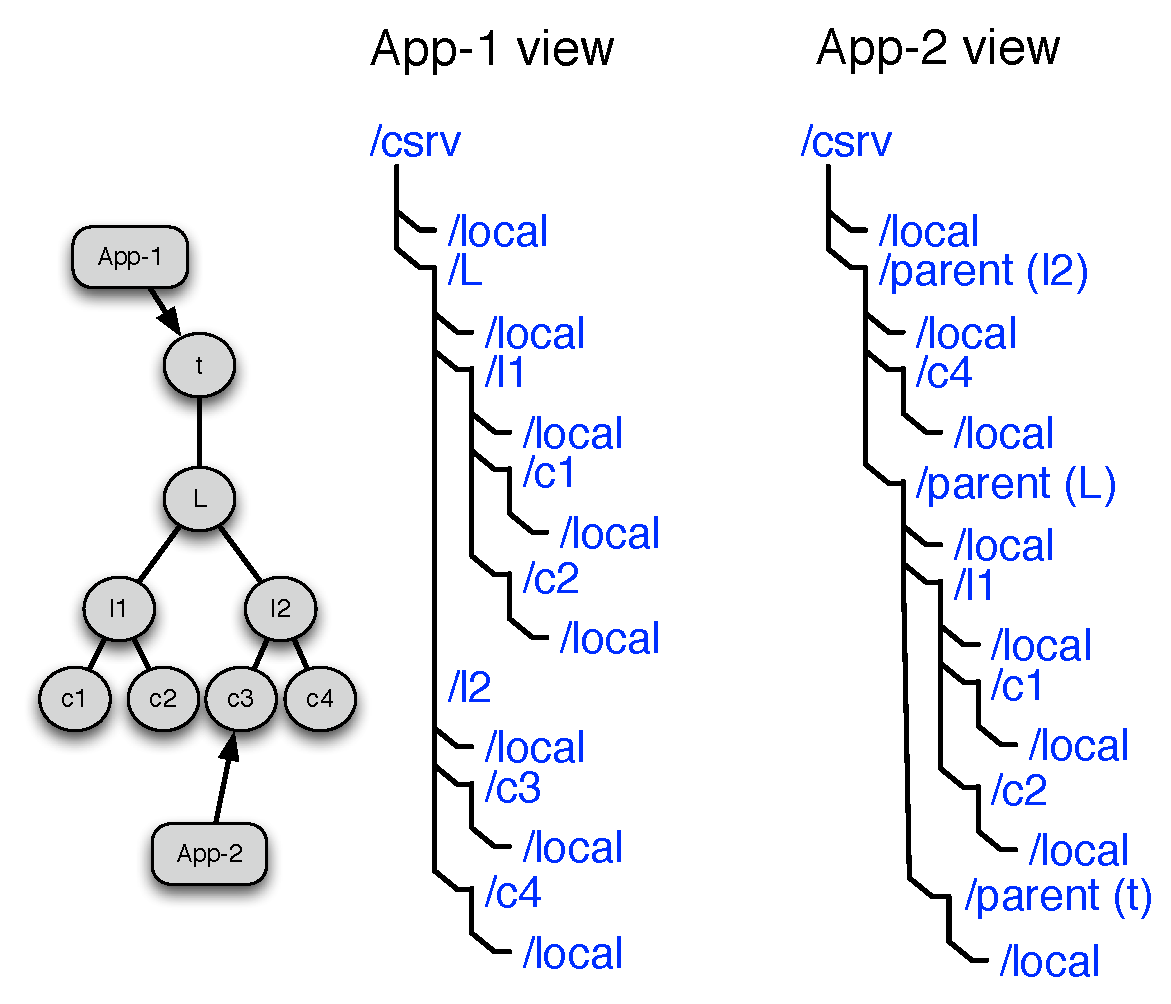
\includegraphics[width=3in]{./img/csrv-views.eps}
\caption{Sample filesystem interface for sample the topology in Brasil}
\label{fig:xcpu3FSTopo}
\end{figure}

Assuming the links between the nodes are created by the remote node mounts in
central services, this diagram shows how the filesystem views at different
nodes encompasses the whole network, even though each node is only connected to
its neighbours. The Brasil filesystem starts with the \texttt{[/csrv]}
directory. The location \texttt{[/csrv/local/]} presents the local resources
whereas \texttt{[/csrv/parent/]} presents the Brasil filesystem of the parent
node. All other directories in the represents the Brasil filesystem of the
children nodes.  It can be easily seen that both \textit{App-1} and
\textit{App-2} have access to all the nodes even though they are running on
different nodes.  In this design, every node has to worry about only its
children and the parent, other topology falls into place automatically.

Just because every node can construct the global view, does not mean that it
must use this global view for making any decision or performing a typical
operation. The nodes mostly use only the local view for decision making and
operations. This local view includes the parent node and the children nodes.


